\begin{figure*}[thp]
	\center
	\begin{subfigure}{0.7\textwidth}
		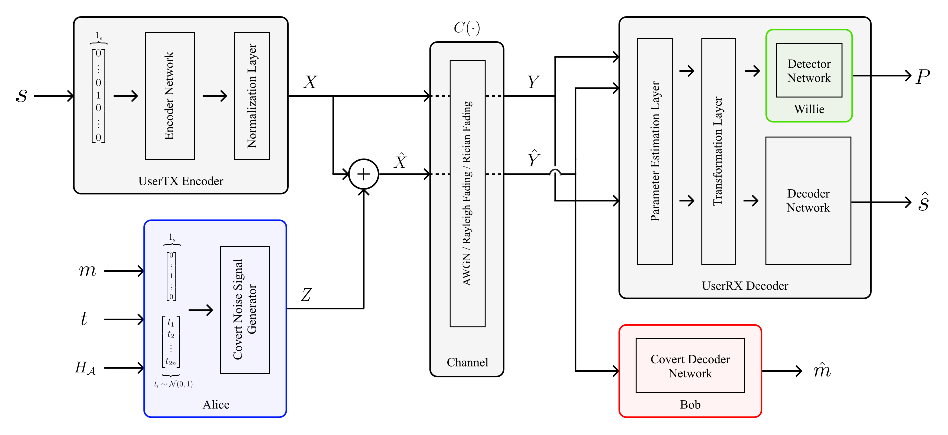
\includegraphics[width=\linewidth]{figs/system_architecture}
	\end{subfigure}
	\\
	\caption{Overall architecture of our system model in the single-user scenario. The UserTX uses an encoder network to encode binary messages into a vector of signals. Alice also transmits her covert signals into the shared channel. After passing through the channel, the UserRX extracts the normal message, Bob decodes the covert message, and Willie attempts to distinguish covert and normal signals from the signals. Components controlled by the covert users are colored, while non-controllable parts of the system are gray.)}	
	\label{fig:system_architecture}
\end{figure*}


\section{System Model}
\label{s:single-model}
In this section, we provide an overview of the system and define each actor's role in our system model.

Our system consists of normal users who communicate with each other via autonencoder wireless systems. This communication can be either single-user, i.e., communication between a single pair of a transmitter and a receiver, or multi-user, i.e., communication between multiple transmitters and a base station receiver. In the single-user setup, we refer to the encoder or the transmitter as UserTX, and to the decoder or the receiver as UserRX. In the multi-user system, on the other hand, there are multiple transmitters (UserTXs) that communicate with a single base station (BaseRX), which acts as a central receiver. These transmitters each use their own encoder network to encode a binary message to a vector of signals. Their networks share no parameters and have no knowledge of other transmitters' messages. Each and every pair of UserTX and BaseRX forms an autoencoder model, with UserTX representing the encoder and BaseRX accounting for the decoder network.
In both single and multi-user systems, communication begins with UserTX encoding a binary message to a vector of signals using its encoder network. This vector of signals is then transmitted over the channel. We consider three channel models of AWGN, Rayleigh fading, and Rician fading. In the case of the multi-user system, as transmitters send their signals simultaneously over a shared channel, there will be interference at the receiver. In the end, a noisy version of the transmitted signal is received at the receiver side, where UserRX or BaseRX extracts the message(s) by decoding the signals. In the multi-user setup, BaseRX receives the signals from all transmitters using multiple antennas and decodes the messages in the same way UserRX does. The only difference is that BaseRX handles the decoding process not just for one, but for all the transmitters' signals in one pass.
In the case of fading channels, before the receiver passes the signals to the decoder network, it equalizes them using the channel matrix. This channel matrix is estimated by the receiver in the single-user system and provided to the decoder in the multi-user system. Figures \ref{fig:system_architecture} and \ref{fig:multi_system_architecture} show an overview of our system model in both single-user and multi-user scenarios.

On the other hand, we have the covert user whose objective is to establish hidden communication in the above system without arousing suspicion from the observer. There is a covert sender (Alice) who wants to communicate secretly with her intended receiver (Bob). Bob is an adversary access point, and his existence is no secret to the other entities in the system. However, if anyone tries to secretly communicate with him, the system's observer (Willie) will mitigate their communication and shut it down. Willie listens to all ongoing transmissions on the channel and uses a binary classifier network to determine the likelihood of each signal being covert or normal. Any distortion in the normal signals can alert Willie to the presence of a covert transmission, so Alice must carefully select her covert signals. This means she should not make any noticeable changes to the statistical properties of the channel noise or the other normal signals. The covert signals should also not increase the error rate of the system, as an unexpected increase in the error rate can raise suspicion. We consider Willie to be an integrated module at the receiver of the normal communication system, i.e., UserRX in the single-user and BaseRX in the multi-user system. This way, he can not only detect incoming covert signals but also measure the communication's error rate. We represent all these three roles with DNNs that are put in a training setup similar to GANs. An adversarial training setting as such ensures that the optimal solution is only achieved when all three reach equilibrium at the end of training.

The covert communication starts with Alice using her generative model to embed a confidential message into a covert noise vector. In non-fading channels, Alice merely needs a covert message and a random trigger to produce a covert signal. However, in fading channels, she requires the channel state information of her channel to Bob in the single-user system, and also the channel state information from other users to Bob in the multi-user system. Bob can provide this information to Alice by listening to the broadcasted pilot signals of other transmitters and measuring the channel state. Since Bob's existence need not be hidden, he can freely broadcast this information as an access point. Next, Alice produces the signals and transmits them into the shared channel, irrespective of other users' transmissions. This means that her covert signals should be agnostic to the normal signals. After getting mixed with other users' transmissions and distorted by the channel effects, Bob receives this signal and extracts Alice's message from it. Unlike the receiver or the observer, here we assume that Bob has only one antenna at his receiver. To keep their communication hidden from Willie, Alice and Bob incorporate a statistical undetectability constraint on the produced covert signals by optimizing their transmissions against his network. When Willie's classifier can do almost no better than random guessing in detecting covert and normal signals, we can safely assume that low probability of detection covert communication has been achieved.

\begin{figure*}[thp]
	\center
	\begin{subfigure}{0.7\textwidth}
		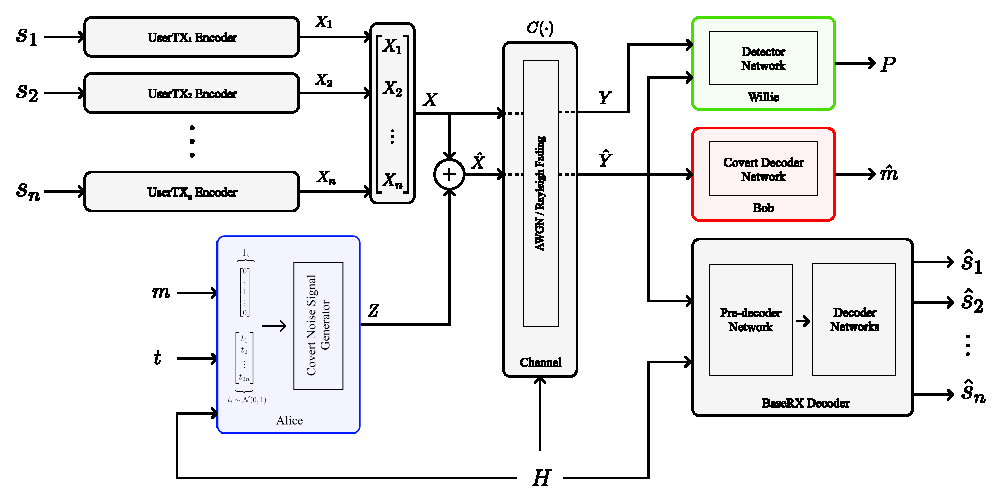
\includegraphics[width=\linewidth]{figs/multi_system_architecture}
	\end{subfigure}
	\\
	\caption{The overall architecture of our system model in the multi-user scenario. Each UserTX separately encodes binary messages into a vector of signals. Meanwhile, Alice transmits her covert signals into the shared channel. After passing through the channel, BaseRX extracts the normal messages, Bob decodes the covert message, and Willie tries to distinguish between covert and normal signals. The colored components in the system are under the control of the covert users, while the gray components are non-controllable parts of the system.}
	\label{fig:multi_system_architecture}
\end{figure*}

\section{GAN-Based Covert Model}
For a given binary secret message \(m\), Alice first applies a one-hot encoding technique, and then utilizes her generator model to produce a covert noise signal \(Z\). With this stochastic generative model, each covert message is mapped to a set of different covert noise signals instead of a single one. Alice then sends this covert signal to the shared channel, which is accessible to all entities within the system. This covert signal mixes with the signals \(X\) from other normal tranmsitters and forms a mixed covert signal \(\hat{X}\). 

\begin{equation}
	\hat{X} = X + Z.
\end{equation}

As previously mentioned, we consider three channel models: AWGN, Rayleigh fading, and Rician fading. Therefore, there will be three different channel outputs for these three channel models. We use a mapping function \(\mathcal{C}(\cdot)\) to express each of these channels' outputs. Since signals in the multi-user system also experience interference, we express single-user and multi-user channel's outputs separately.

\textit{AWGN Channel Output}: For the AWGN channel model, the signal received at the receiver carries the channel's noise effect \(N \sim \mathcal{N}(0, \sigma^2)\). Consequently, the channel function \(\mathcal{C}(\cdot)\) and the final covert signal \(\hat{Y}\) in the single-use system can be represented as:
\begin{equation}
	\hat{Y} = \mathcal{C}(\hat{X}) = X + Z + N.
\end{equation}
For the multi-user system, signals also get distorted by the channel interference effect. This is due to the multiple transmitters sending their signals at the same time. Consequently, the resulting covert signal can be denoted as:
\begin{equation}
	 \hat{Y} = \mathcal{C}(\hat{X}) = \sum^{i \in U}X_i + Z + N.
\end{equation}
where \(U\) is the set that contains all transmitters.

\textit{Rayleigh and Rician Fading Channel Outputs}: We consider a flat-frequency block-fading channel model for Rayleigh and Rician fading, where each signal vector (codeword) is assumed to be faded independently. Let \(H_{\mathcal{U}}\) be the fading coefficient for the signal vector \(X\), and \(H_{\mathcal{A}}\) be the fading coefficient for Alice's signal. The channel function \(\mathcal{C}(\cdot)\) and the resulting covert signal \(\hat{Y}\) in the single-user system are given by:
\begin{equation}
	\hat{Y} = \mathcal{C}(\hat{X}) = (H_{\mathcal{U}} \cdot X) + (H_{\mathcal{A}} \cdot Z) + N.
\end{equation}

In the multi-user case, the final covert signal including the channel interference can be written as:
\begin{equation}
	\hat{Y} = \mathcal{C}(\hat{X}) = \sum^{i \in U}(H_{\mathcal{U}_i} \cdot X_i) + (H_{\mathcal{A}} \cdot Z) + N.
\end{equation}

On the receiving end, Bob receives the distorted covert signal \(\hat{Y}\) and uses his decoder network to reconstruct the covert message \(\hat{m}\).

Willie's network captures the statistical properties of signals transmitted over the channel. Its objective is to classify sequences of normal signals \(Y\) and covert signals \(\hat{Y}\) while providing useful feedback to Alice during training. This feedback helps Alice modify the produced covert signals such that they are indistinguishable from the normally transmitted signals. This ensures that when the model is deployed in a real communication setup, it is highly unlikely for any observer to detect the covert transmissions.

\subsection{General Formulation}
\textbf{Reliability}: The first objective of our covert model is to enable reliable covert communication. In order to achieve this, Bob needs to be able to accurately decode the covert messages that Alice sends through the covert signals \(\hat{Y}\). As mentioned earlier, Alice employs a generative model to produce covert noise signals that correspond to the covert messages. Let \(\Theta_{\mathcal{A}}(\cdot)\) be the underlying function of Alice's generative model that takes a random trigger \(t \sim \mathcal{N}(0, 1)\), a covert message \(m\), the channel coefficients from Alice to Bob \(H_{\mathcal{A}}\), and in the multi-user system, the channel matrix \(H_{\mathcal{U}}\) and produces a covert signal \(Z\). The corresponding covert signal can be denoted as \(Z_{m, t} = \Theta_{\mathcal{A}}(m, t, H_{\mathcal{A}}\footnotemark[1]), H_{\mathcal{U}}\footnotemark[2])\)). Let  \(\Theta_{\mathcal{B}}(\cdot)\) be the underlying function of the decoder network that Bob uses to reconstruct the covert message \(\hat{m}\). Then the reliability of communication between Alice and Bob is achieved using the following loss function:
\begin{equation}
	\begin{aligned} \label{bob_loss}
	\mathcal{L}_{\mathcal{B}} & = \mathbb{E}_{m}[\mathcal{H}(\hat{m}, m)] \\
	& = \mathbb{E}_{m}[\mathcal{H}(\Theta_{\mathcal{B}}(\hat{Y}), m)] \\ 
	& = \mathbb{E}_{m}[\mathcal{H}(\Theta_{\mathcal{B}}(\mathcal{C}(\hat{X}), m)] \\ 
	& = \mathbb{E}_{m}[\mathcal{H}(\Theta_{\mathcal{B}}(\mathcal{C}(\Theta_{\mathcal{A}}(m, t, H_{\mathcal{A}}) + X)), m)].
	\end{aligned}
\end{equation}
For the multi-user system, this equation is written as:
\begin{equation}
	\begin{aligned}
		\mathcal{L}_{\mathcal{B}} & = \mathbb{E}_{m}[\mathcal{H}(\hat{m}, m)] \\
		& = \mathbb{E}_{m}[\mathcal{H}(\Theta_{\mathcal{B}}(\mathcal{C}(\Theta_{\mathcal{A}}(m, t, H_{\mathcal{A}}, H_{\mathcal{U}}) + X)), m)].
	\end{aligned}
\end{equation}
The equation above uses the cross-entropy function \(\mathcal{H}(\cdot)\) to measure the difference between the probability of the reconstructed covert message \(\hat{m}\) nd the actual covert message \(m\). This equation can be used to optimize the networks of both Alice and Bob by freezing one or the other's network parameters iteratively.

\footnotetext[1]{This is an extra input parameter that is only used in the systems with fading channel.}
\footnotetext[2]{This is an extra input parameter that is only used in the multi-user system with fading channel.}

\textbf{Low Interference}: Although (\ref{bob_loss}) ensures communication accuracy, it is also necessary to ensure that the generated perturbations do not negatively impact normal communication between UserTX and UserRX. Otherwise, this could alert Willie to abnormal activity. To address this, we add a constraint that minimizes UserRX's loss function during Alice's training. In a single-user system, we can express this constraint as follows:
\begin{equation}
	\begin{aligned} \label{alice_user_loss}
	\mathcal{L}_{\mathcal{U}} & = \mathbb{E}_{m}[\mathcal{H}(\hat{s}, s)] \\
	& = \mathbb{E}_{m}[\mathcal{H}(\Theta_{\mathcal{U}}(\hat{Y}), s)] \\
	& = \mathbb{E}_{m}[\mathcal{H}(\Theta_{\mathcal{U}}(\mathcal{C}(Z + X)), s)] \\
	& = \mathbb{E}_{m}[\mathcal{H}(\Theta_{\mathcal{U}}(\mathcal{C}(\Theta_{\mathcal{A}}(m, t, H_{\mathcal{A}}) + X)), s)].
	\end{aligned}
\end{equation}
where \(\Theta_{\mathcal{U}}(\cdot)\) refers to UserRX's decoder network function. It is important to note that during this training, UserRX's decoder network is frozen and only Alice's parameters will be updated.

For the multi-user system, since we have multiple transmitters sending signals, we need to minimize BaseRX's loss function over all individual transmitters' signals. Thus, equation \ref{alice_user_loss} is rewritten as follows:
\begin{equation}
	\begin{aligned} \label{multi_alice_user_loss}
		\mathcal{L}_{\mathcal{U}} & = \sum^{i \in U}\mathbb{E}_{m}[\mathcal{H}(\hat{s}_i, s_i)] \\
		= \sum^{i \in U} & 
			\mathbb{E}_{m}[\mathcal{H}
			((\Theta_{\mathcal{U}}(\mathcal{C}(\Theta_{\mathcal{A}}(m, t, H_{\mathcal{A}}, H_{\mathcal{U}}) + X_i),  H_{\mathcal{U}}), s_i)].
	\end{aligned}
\end{equation}

\begin{algorithm}[tp!]
	\caption{Optimizing covert models algorithm}\label{alg:cap}
	\small
	\begin{algorithmic}
		\State $X \gets$ normal signals data
		\State $S, M \gets$ normal and covert messages sets
		\State $\Theta_{\mathcal{A}}, \Theta_{\mathcal{B}}, \Theta_{\mathcal{W}} \gets$ Alice, Bob, and Willie network functions
		\State $\Theta_{\mathcal{U}} \gets$ UserRX decoder network function
		\State $\mathcal{H} \gets$ cross entropy function
		\State $\mathcal{C} \gets$ channel mapping function
		\For{epoch $ep \in \{1 \ldots n_{epochs}$\}}
		\State $t \sim \mathcal{N}(0, 1)$
		\State $\mathcal{L}_{\mathcal{W}} = \mathcal{H}(\mathcal{C}(X), \mathcal{C}(\Theta_{\mathcal{A}}(M, t, H_{\mathcal{A}}, H_{\mathcal{U}}) + X))$
		\State Update $\Theta_{\mathcal{W}}$ to minimize $\mathcal{L}_{\mathcal{W}}$
		\State $\mathcal{L}_{\mathcal{B}} = \mathcal{H}(\mathcal{C}(\Theta_{\mathcal{A}}(M, t, H_{\mathcal{A}}, H_{\mathcal{U}}) + X), M)$
		\State Update $\Theta_{\mathcal{B}}$ to minimize $\mathcal{L}_{\mathcal{B}}$
		\State $\mathcal{L}_{\mathcal{U}} \gets \mathcal{H}(\Theta_{\mathcal{U}}(\mathcal{C}(\Theta_{\mathcal{A}}(M, t, H_{\mathcal{A}}, H_{\mathcal{U}}) + X)), S)$
		\State
		$\mathcal{L}_{\mathcal{A}} = \lambda_{\mathcal{B}} \mathcal{L}_{\mathcal{B}} + \lambda_{\mathcal{U}} \mathcal{L}_{\mathcal{U}} - \lambda_{\mathcal{W}} \mathcal{L}_{\mathcal{W}}$
		\State Update $\Theta_{\mathcal{A}}$ to minimize $\mathcal{L}_{\mathcal{A}}$
		\EndFor
	\end{algorithmic}
\end{algorithm}

\textbf{Undetectability}: In our model, Willie acts as a critic network, similar to what is known as a discriminator in GAN models \cite{goodfellow2014generative}. The so-called real and fake samples in GANs' discriminator training process here are mapped to normal and covert signals, respectively. For the single-user system, we use the following loss function to optimize Willie's network that classifies covert and normal signals:
\begin{equation}
	\begin{aligned} \label{willie_loss}
	\mathcal{L}_{\mathcal{W}} & = \mathbb{E}_{m}[\mathcal{H}(\hat{y}, y)] \\
	& = \mathbb{E}_{m}[\mathcal{H}(\mathcal{C}(\hat{X}), \mathcal{C}(X))] \\
	& = \mathbb{E}_{m}[\mathcal{H}(\mathcal{C}(\Theta_{\mathcal{A}}(m, t, H_{\mathcal{A}}) + X), \mathcal{C}(X))].
	\end{aligned}
\end{equation}
where \(\mathcal{H}(\cdot)\) is the binary cross entropy between the covert signals \(\hat{Y}\) and the normal signals \(Y\). For the multi-user system, we need to optimize the Willie's network over all the transmitters' outputs.

\begin{equation}
	\begin{aligned} \label{multi_willie_loss}
		\mathcal{L}_{\mathcal{W}} & = 
		\sum^{i \in U} \mathbb{E}_{m}[H(\hat{Y}, Y)] \\
		& = \sum^{i \in U}
			\mathbb{E}_{m}[\mathcal{H}(\mathcal{C}(\Theta_{\mathcal{A}}(m, t, H_{\mathcal{A}}, H_{\mathcal{U}}) + X), \mathcal{C}(X))].
	\end{aligned}
\end{equation}

This white-box adversarial training against Alice's network ensures that Willie's network will be adequately trained to distinguish between covert and normal signals. On the other hand, we do not want the covert signals produced by Alice to deviate from the statistical properties of the normal signals on the channel, as this would increase the likelihood of the observer detecting and mitigating the covert communication. To achieve this undetectability property, we use Willie's network to act as a discriminator network in Alice's optimization function. In other words, Alice's training against this network aims to maximize Willie's uncertainty about his predictions. This regularizer helps Alice and Bob form their covert communication in a way that is indistinguishable from the actual channel's noise, yet understandable by both. Overall, Alice's loss function can be expressed as a weighted sum of these three objectives:
\begin{equation}
	\begin{array}{l} \label{alice_loss}
	\mathcal{L}_{\mathcal{A}} = \lambda_{\mathcal{B}} \mathcal{L}_{\mathcal{B}} + \lambda_{\mathcal{U}} \mathcal{L}_{\mathcal{U}} - \lambda_{\mathcal{W}} \mathcal{L}_{\mathcal{W}}.
\end{array}
\end{equation}
where \(\lambda_{\mathcal{B}}\), \(\lambda_{\mathcal{U}}\), and \(\lambda_{\mathcal{W}}\) are hyperparameters that determine the relative importance of the different objectives in Alice's loss function. The algorithmic steps involved in training our covert models are summarized in Algorithm \ref{alg:cap}

\begin{figure*}[!tp]
	\center
	\begin{subfigure}{0.28\textwidth}
		\includegraphics[width=\linewidth]{figs/autoencoder_bler_awgn}
		\caption{AWGN channel}
	\end{subfigure}
	\begin{subfigure}{0.28\textwidth}
		\includegraphics[width=\linewidth]{figs/autoencoder_bler_rician}
		\caption{Rician fading channel}	
	\end{subfigure}
	\begin{subfigure}{0.28\textwidth}
		\includegraphics[width=\linewidth]{figs/autoencoder_bler_rayleigh}
		\caption{Rayleigh fading channel}	
	\end{subfigure}
	\caption{Autoencoders' performance in terms of BLER over a range of SNR values is evaluated in our single-user system. The models are trained over AWGN, Rayleigh, and Rician fading channels for a set of parameters that have the same data rate.}
	\label{fig:autoencoder_bler}
\end{figure*}

\subsection{Neural Network Architecture}
\textbf{User's Autoencoder Network}: The autoencoder model takes in a binary message \(s\) of size \(k\) bits and outputs a reconstructed version of it, denoted by \(\hat{s}\). The encoder maps the message to a vector of signals of size \(2 \times n\), where \(n\) is the number of channel uses, using one-hot encoding. Since there are multiple encoders in the multi-user system, the resulting vector will have a size of \(n_{tx} \times (2 \times n)\). The signals generated from the encoder are then passed to the channel mapping function, which incorporates the channel noise and interference effects. When the system is single-user and there is fading in the channel model, the receiver side utilizes the two layers of parameter estimation and transformation to equalize the signals. We apply a simple transformation function that divides signals by the channel fading coefficients estimated via the parameter estimation layer. Note that more complex transformation functions can be used, as described in \cite{o2017introduction}; however, optimizing the performance of the autoencoder model is out of the scope of this article. For the multi-user system, the decoder is provided with channel coefficients as input. This enables BaseRX to use the zero-forcing technique \cite{garg2010wireless} to equalize the received signals. In the case of a single-user system, UserRX utilizes its decoder network to reconstruct the message. However, in the multi-user system, BaseRX receives signals from all transmitters and simultaneously decodes them. This is achieved by first passing the signals to a pre-decoder network and then using separate decoders at the final layers.


\textbf{Alice's Network}: Alice first transforms a covert message \(m\) to its corresponding one-hot encoding representation, where each message belongs to a unique class. She then uses a random trigger \(t\) to randomize the process by which the covert noise signal \(Z\) is produced, along with the channel coefficients \(H_{\mathcal{A}}\) and \(H_{\mathcal{U}}\). For Alice's generator model, we use multiple dense layers with ReLU and Tanh activation functions. The first layer acts as an embedding layer, enlarging the input's domain space. The subsequent fully connected layers extract useful features and perform the encoding process. Finally, the last layer performs a dimension transformation, ensuring that the generated covert signal \(Z\) complies with the dimension of the normal signal \(X\) on the channel. 


\textbf{Bob's Network}: Bob receives the covert signal \(\hat{Y}\) that has been affected by the channel, and he feeds it through his decoder network to extract the secret message. Bob's network is more sophisticated than Alice's, as decoding such a distorted signal is a much more complex task. The received message first goes through a wide dense layer with a Tanh activation function, which increases the input's feature space. The data then passes through multiple 1-Dimensional Convolutional (1D Conv) layers, which learn the coding that Alice has developed to encode the covert messages. We have found that using 1D Conv layers helps Bob and Alice achieve better consistency in the accuracy of their communication, especially when the channel model is more complicated (i.e., when there is also fading in the channel). The rest of Bob's decoder network consists of two dense layers that remap the learned feature space to the covert message domain space. As with UserRX's and BaseRX's decoder networks, Bob eventually predicts the covert message by performing a classification on the received signal.


\textbf{Willie's Network}: Willie's task is to distinguish between the normal signal  \(Y\) and the covert  signal \(\hat{Y}\). To achieve this, he uses a neural network with the same architecture as Bob's, except for the last layer, which has a Sigmoid activation function instead of Softmax. The network takes both normal and covert signals as inputs and outputs a confidence probability \(P\) indicating the likelihood of the signal being normal. Using the same network architecture for both Bob and Willie ensures a fair competition between them, as they have the same capacity for training.